\subsection{Inicialización}
En ésta fase se describirá la linea base sobre la que se desarrollará el proyecto, esto significa, definir las herramientas y dispositivos con los que se realizará el desarrollo y testing, qué tecnologías vamos a usar y el planteamiento general del sistema.\par
\noindent
\\
\textbf{Herramientas y Tecnologías}:
	\begin{itemize}
			\item \textbf{Amazon Web Services.} Amazon Web Services (AWS) es una infraestructura de servicios en la nube usados para el desarrollo de sistemas. AWS tiene una gran cantidad de servicios útiles para el desarrollo de ARF de los cuales se usarán los siguientes para el desarrollo de ARF: S3 (almacenamiento), RDS (base de datos), Lambda (ejecución de código en la nube), API Gateway (comunicación con Lambda via internet).
			\item \textbf{Android 8 Oreo y Android 7 Nougat.} Estas son las versiones de Android que son compatibles con ARCore 1.5
			\item Android Studio 2.19
			\item \textbf{ARCore 1.5.} Es una librería para el desarrollo de aplicaciones con realidad aumentada de Google. Tras las pruebas de contexto se eligió usar ARCore en su versión 1.5 que es la versión estable más actual.
			\item \textbf{Blender 2.79.} Es un modelador y renderizador de objetos en 3D. Se usará para las primeras integraciones de ARCore donde utilizaremos modelos 3D de elaboración propia.
			\item \textbf{GitHub.} Es un sistema de control de versiones que sirve para tener el código fuente centralizado en repositorios y que varias personas puedan actualizar simultáneamente el código de forma rápida y sencilla. El código de ARF estará alojado en un repositorio de GitHub.
			\item \textbf{Git.} Es un cliente usado para la integración de GitHub en plataformas como Windows y GNU-Linux. Se usará para realizar la comunicación con GitHub.
	  		\item \textbf{JSON.} Es un formato para la estructuración de datos. Se usará debido a su facilidad de uso e integración con AWS.
	\end{itemize}
	\noindent
\textbf{Dispositivos}:
\begin{itemize}
	\item \textbf{Laptop.} Marca Acer, procesador Intel Core i3 6ta generación, 4GB de RAM, 1TB en disco duro, S.O. Debian 9.5
	\item \textbf{Laptop.} Marca HP, procesador Intel Core i5 6ta generación, 4GB de RAM, 1TB en disco duro, S.O. Windows 10
	\item \textbf{PC} Procesador AMD Ryzen 7 1800X, 16GB de RAM, 1TB en disco duro, S.O. Windows 10
	\item \textbf{Móvil.} Moto G6, procesador Snapdragon 450 a 1.8GHz, 3GB de RAM, 32GB de almacenamiento, S.O. Android 8.0
	\item \textbf{Móvil.} Moto G6+, procesador Snapdragon 630 a 2.2GHz, 4GB de RAM, 32GB de almacenamiento, S.O. Android 8.0	
\end{itemize}
\noindent
\textbf{Arquitectura}:
El backend de la aplicación se encontrará sobre la infraestructura de Amazon Web Services (AWS), debido a la alta escalabilidad que proporciona. La arquitectura contendrá un cluster RDS con MySQL, nueve Lambdas, un Bucket de S3 y una API Gateway (véase Figura 4.25).\par
A continuación se describe el funcionamiento de cada Lambda:\par
\begin{itemize}
	\item\textbf{ARFLogin}. Contiene toda la lógica y la seguridad informática relacionada con la autenticación en la aplicación.
	\item\textbf{ARFRegister}. Permitirá registrar una nueva cuenta en el sistema, misma que permitirá guardar proyectos y escenarios.
	\item\textbf{ARFRecoverAccount}. Esta Lambda contendrá la lógica para poder reestablecer la contraseña de una cuenta, para el caso en el que un usuario olvide su contraseña.
	\item\textbf{ARFProject}. Contiene la lógica para poder crear, obtener, actualizar y eliminar proyectos.
	\item\textbf{ARFAssets}. Contiene la lógica para poder crear, obtener, actualizar y eliminar muebles incluyendo los modelos 3D de los mismos.
	\item\textbf{ARFGetScenario}. Permite obtener un escenario específico o los escenarios de un usuario en particular.
	\item\textbf{ARFStoreScenario}. Esta función se encarga de guardar los escenarios generados en la aplicación, incluyendo sus fotografías. Los videos no son manipulados por esta Lambda puesto que se almacenarán localmente en los dispositivos móviles, debido a su gran tamaño lo cual implica un largo tiempo de subida a la nube.
	\item\textbf{ARFUpdateScenario}. Contiene la lógica para poder actualizar la información general de los escenarios. También se encarga de eliminar fotografías de los escenarios, pero no agregar nuevas, debido a que las fotografías se generan únicamente durante la creación de un escenario.
	\item\textbf{ARFDeleteScenario}. Permite eliminar escenarios previamente creados.
\end{itemize}
\noindent
Las Lambdas por sí solas sólo pueden comunicarse entre la misma infraestructura de AWS, pero no al exterior, para ello se requiere el servicio API Gateway que permite que las Lambdas puedan tener comunicación con el mundo exterior a través del protocolo HTTPS. Funciona de la siguiente manera:
\begin{itemize}
	\item Se envía una petición a una URL de consumo de la API Gateway con un cuerpo de mensaje en formato JSON.
	\item La API Gateway se encarga de enviar el mensaje a una Lambda, dependiendo de la URL de consumo que fue empleada.
	\item La API Gateway se queda esperando a que la Lambda termine de ejcutarse.
	\item La Lambda recibe el mensaje en formato JSON y se ejecuta. Dependiendo de lo que esté programado en la función, puede conectarse a S3 o a una instancia de MySQL. Cuando finaliza su ejecución, devuelve una respuesta a la API Gateway.
	\item La API Gateway recibe esta respuesta y se encarga de devolverla al cliente que realizó la petición.
\end{itemize}

De esta forma la app puede comunicarse con AWS y obtener los recursos que necesite para realizar sus funciones.\par
Además de la aplicación móvil, existe una plataforma web que se encuentra como app de Google Firebase. El objetivo de esta plataforma es que los usuarios registrados puedan entrar a su cuenta y agregar muebles (incluyendo sus modelos 3D) los cuales podrán ser usados en la aplicación, de tal forma que si algún diseñador de interiores desea visualizar un mueble especifico en el entorno de realidad aumentada, pueda agregarlo desde la plataforma web de ARF. Dentro de la misma plataforma será posible visualizar los modelos 3D.


\begin{figure}[H]
	\centering
	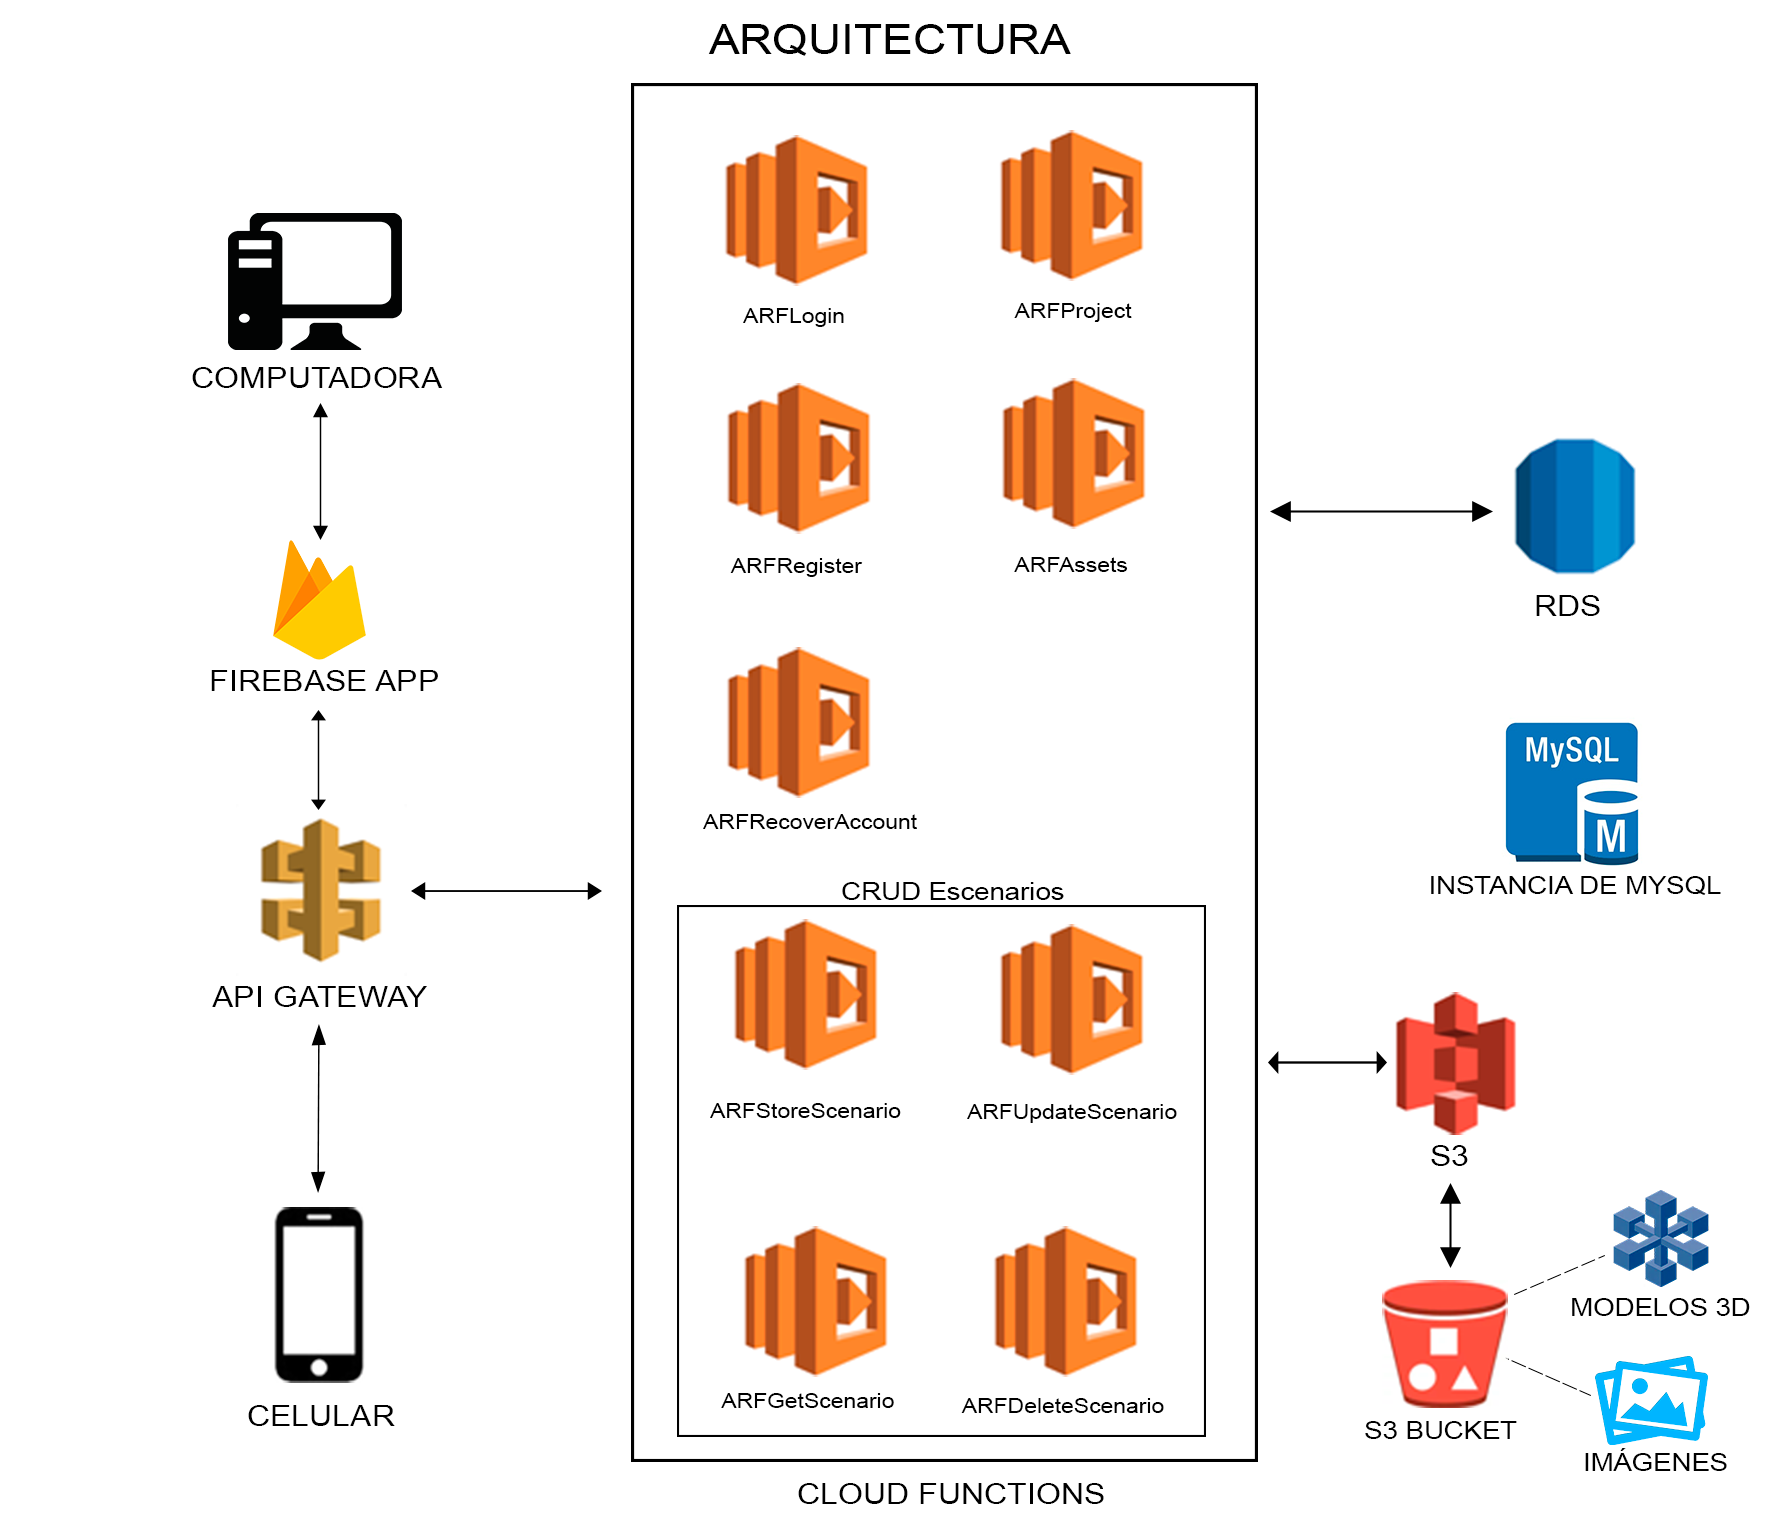
\includegraphics[width=15cm,height=15cm]{imagenes/desarrollo/arquitectura/ArchitecturaBackend.png}
	\caption{Arquitectura de Backend de ARF.}
	\label{fig:arqbackend}
\end{figure}
\par
Por otro lado se requerirá una base de datos que pueda almacenar los usuarios, proyectos, escenarios, categorías y subcategorías que se vayan generando. Para el tipo y cantidad de información que se requiere almacenar, una base de datos relacional en tercera forma normal cumple a ésta necesidad. En las figuras  3.16, 3.17 y 3.18 se muestra el proceso de normalización la base de datos que se va a usar en ARF, misma que se encuentra en Amazon RDS mostrado en la figura 4.26.
\begin{figure}[H]
	\centering
	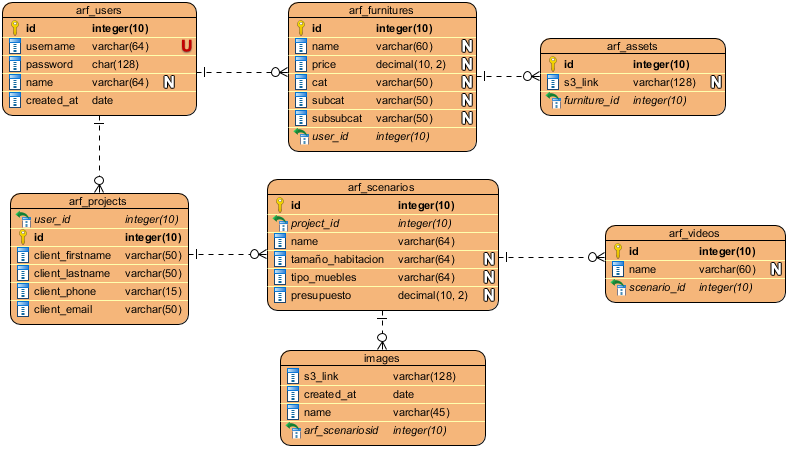
\includegraphics[width=16cm,height=8cm]{imagenes/desarrollo/arquitectura/ERD.png}
	\caption{Primera forma normal de la base de datos de ARF.}
	\label{fig:erd1}
\end{figure}
\begin{figure}[H]
\centering
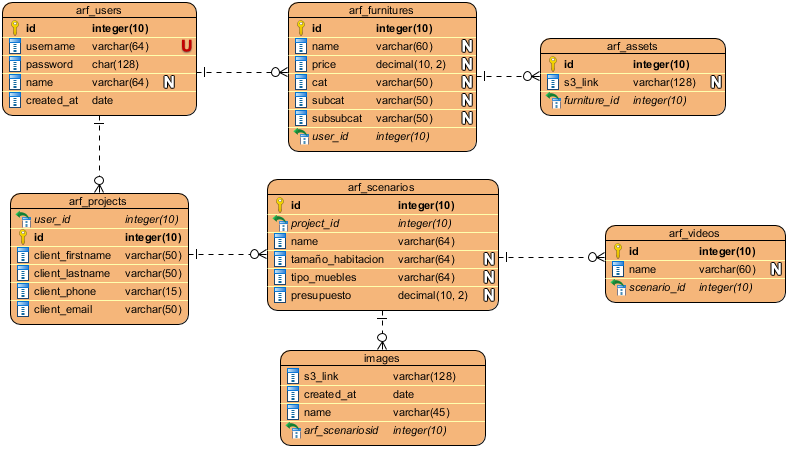
\includegraphics[width=16cm,height=8cm]{imagenes/desarrollo/arquitectura/ERD.png}
\caption{Segunda forma normal de la base de datos de ARF.}
\label{fig:erd2}
\end{figure}
\begin{figure}[H]
\centering
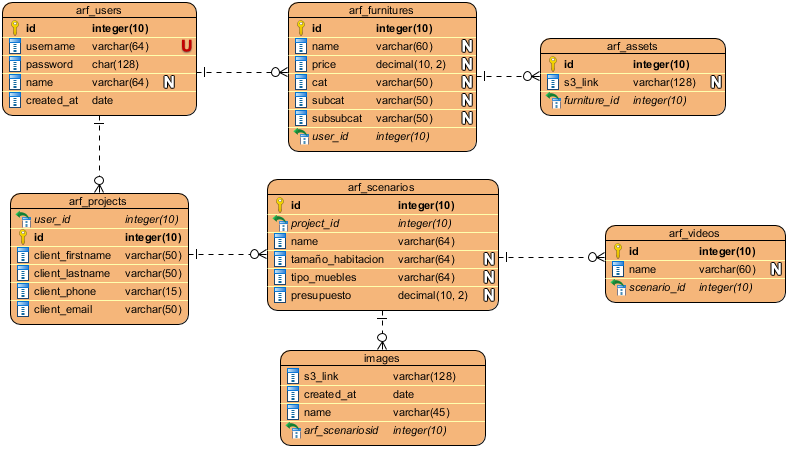
\includegraphics[width=16cm,height=8cm]{imagenes/desarrollo/arquitectura/ERD.png}
\caption{Tercera forma normal de la base de datos de ARF.}
\label{fig:erd}
\end{figure}